\chapter{Scope Statement}

\section{Host Company}
\subsection{Converty}
Converty is an advanced platform for building and managing high-converting online stores. Converty provides powerful tools and advanced features that enable business owners and merchants to create effective online stores without the need for programming skills.

\begin{figure}[h]
  \centering
  
\includegraphics[width=0.3\textwidth]{Images/convertyLogo.jpeg}
  \label{fig:Converty Logo}
\end{figure}

The platform offers a variety of services including online store management, customer relationship management (CRM), marketing automation, and reporting tools. Converty's mission is to enhance the e-commerce experience for SMEs by delivering an integrated solution that simplifies operations, reduces costs, and boosts efficiency.
\newline

\subsection{Services}
Converty offers a diverse range of services:
\begin{itemize}
    \item \textbf{Development Team:} Responsible for fixing bugs, adding new features, and optimizing existing functionalities.
    \item \textbf{Marketing Team:} Provides guidance to clients to help them make informed decisions to maximize sales.
    \item \textbf{Support Team:} Ensures customer satisfaction and communicates key information between teams.
\end{itemize}

\section{Study Of The Existing}
Shopify is a popular e-Commerce platform that allows individuals and businesses to create online stores effortlessly. Among its many advantages are the performant templates that ensure fast loading times and a seamless shopping experience for customers.
\newline

In addition to high-performing templates, Shopify offers a variety of sales-boosting features. These include abandoned cart recovery, targeted email campaigns, and advanced analytics. These tools help store owners optimize their online sales and increase revenue.
\newline

Furthermore, Shopify provides a comprehensive mobile app that allows store owners to manage their business on the go. The app includes features like order management, product updates, and sales tracking, making it convenient to maintain an online store anytime, anywhere.

\section{Problem Statement} 
Despite Converty's notable progress in the e-commerce industry, the product currently faces several critical challenges that must be addressed to compete effectively with Shopify. 
\begin{itemize} 
    \item \textbf{Performance Issues:} One of the four templates provided by Converty has performance problems that negatively affect the overall user experience. 
    \item \textbf{Missing Key Features:} The platform lacks essential features such as upselling, which are critical to maximizing sales and improving customer satisfaction. 
    \item \textbf{Incomplete Mobile App Experience:} The mobile app experience is incomplete, limiting accessibility and convenience for users who prefer to manage their online stores on mobile devices. 
\end{itemize} 
Addressing these challenges is crucial for Converty to fully leverage its potential and offer a robust, competitive solution in the e-commerce market.

\section{Proposed Solution}
After a long discussion with the company, the following fixes were decided to be made:

\begin{itemize}
  \item \textbf{Performance Optimization:} The first template will be recoded using React to enhance performance. This will involve refactoring the codebase to improve efficiency and responsiveness, leading to a significantly better user experience.
  \item \textbf{Upsell Feature Integration:} An upsell feature will be added to the platform, incorporating algorithms and interfaces that recommend complementary products to customers. This feature aims to increase the average order value and boost customer satisfaction.
  \item \textbf{Mobile App Enhancements:} Key mobile features will be incorporated to complete the mobile app experience, ensuring a seamless and intuitive user interface for managing online stores on mobile devices.
\end{itemize}

These solutions address the critical issues facing Converty, improving its performance, functionality, and overall user experience in the competitive e-commerce market.
\newline

\section{About the Project}

\subsection{Goals}
The primary goals of this project are to improve the performance of the Converty platform, introduce key features to improve functionality, and complete the mobile app experience to ensure a seamless user interface across all devices.

\subsection{Objectives}
To achieve these goals, the following objectives were set:
\begin{itemize}
    \item Recode the first template using React to enhance performance.
    \item Integrate an upsell feature to boost average order value and customer satisfaction.
    \item Enhance the mobile app with essential features to provide a comprehensive and user-friendly experience.
\end{itemize}

\subsection{Deliverables}
\begin{itemize}
    \item \textbf{Source Code:} The complete source code, including all necessary files for building and running the project. The code should be well organized, adhere to the coding standards, and include comments for clarity.
    \item \textbf{Documentation:} Comprehensive documentation covering the project architecture, major modules, functions, and classes. It should also include setup instructions, usage examples, and relevant information for users and developers.
    \item \textbf{Presentation:} A presentation outlining the project's objectives, design, implementation, key features, challenges, and solutions. It should include visual aids such as diagrams, charts, and screenshots.
\end{itemize}

\subsection{Management Plan}

\subsubsection{Software Development Life Cycle (SDLC)}
The SDLC employed for this project involved iterative development and continuous feedback to meet all project requirements effectively.
\begin{figure}[h]
  \centering
  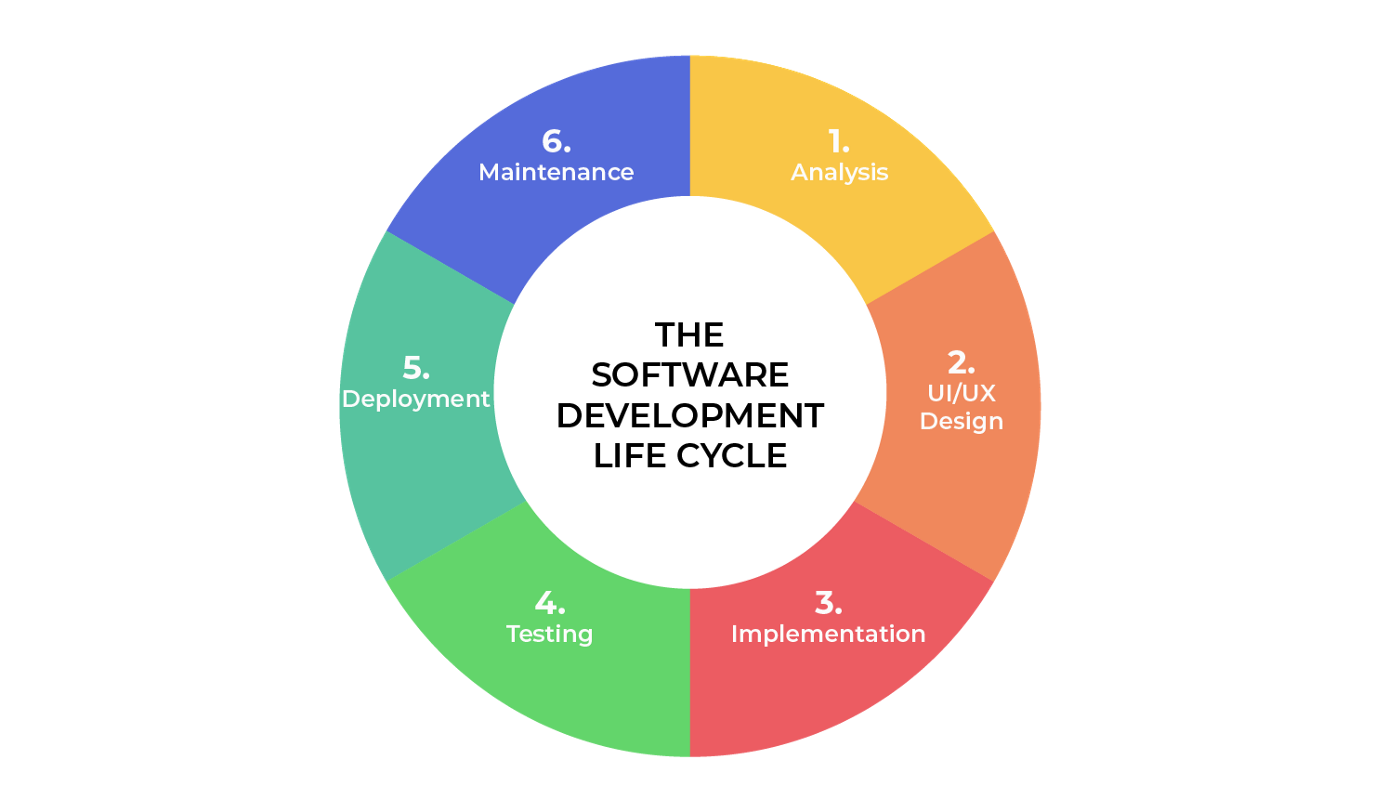
\includegraphics[width=0.6\textwidth]{Images/sdlc.png}
  \caption{SDLC Phases}
  \label{fig:SDLC Phases}
\end{figure}

\subsubsection{Comparison of SDLC Models}

\begin{longtable}{|m{3cm}|m{4cm}|m{4cm}|m{4cm}|}
\hline
\textbf{Model} & \textbf{Advantages} & \textbf{Disadvantages} & \textbf{Suitability} \\
\hline
\endfirsthead
\hline
\textbf{Model} & \textbf{Advantages} & \textbf{Disadvantages} & \textbf{Suitability} \\
\hline
\endhead
Waterfall Model & Simple and easy to understand and use & Inflexible, difficult to make changes once the process is underway & Suitable for small projects with well-defined requirements \\
\hline
Agile Model & Flexible and adaptive to changes, promotes collaboration and customer feedback & Can be difficult to predict effort required and can lead to scope creep & Suitable for projects with dynamic requirements \\
\hline
Scrum Model & Iterative approach promotes continuous improvement, increases team accountability & Requires experienced team members, can be difficult to implement for complex projects & Suitable for complex projects requiring frequent changes \\
\hline
Kanban Model & Visual workflow management, promotes continuous delivery & Lack of time frames can lead to lack of urgency & Suitable for projects needing continuous delivery and improvement \\
\hline
\caption{Comparison of SDLC Models}
\label{tab:sdlc_models}
\end{longtable}

\subsubsection{Agile Methodology}
The Agile methodology emphasizes flexibility, collaboration, customer feedback, and rapid releases. It supports adaptive planning and continuous improvement, making it ideal for dynamic and complex projects. Agile encourages iterative development cycles (sprints) that allow teams to adapt quickly to changing requirements and deliver functional software incrementally.

\subsubsection{Scrum Framework}
The Scrum framework, a subset of Agile, manages complex product development through iterative cycles known as sprints, which typically last 2-4 weeks. Key roles in Scrum include the Product Owner (responsible for project vision and backlog prioritization), the Scrum Master (facilitates the process and resolves issues), and the Development Team (completes the work). Scrum ceremonies such as sprint planning, daily stand-ups, sprint reviews, and retrospectives ensure ongoing progress and improvement.

\begin{figure}[h]
  \centering
  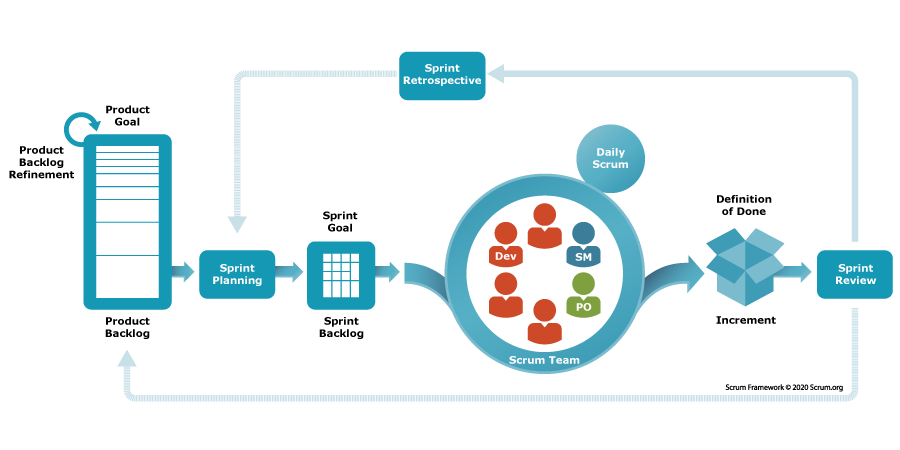
\includegraphics[width=1\textwidth]{Images/scrum.png}
  \caption{Scrum Framework}
  \label{fig:Scrum Framework}
\end{figure}

\subsubsection{Scrum Tools}
To support the Scrum framework, the following tools were utilized:
\begin{itemize}
    \item \textbf{GitHub:} For version control and collaborative code management, allowing team members to work on code simultaneously, track changes, and manage issues.
    \item \textbf{Google Meet:} For virtual meetings including daily stand-ups, sprint planning, reviews, and retrospectives, ensuring remote team members can collaborate effectively.
    \item \textbf{Notion:} An all-in-one workspace for project management, documentation, and collaboration, helping organize tasks, track progress, and maintain a shared knowledge base.
\end{itemize}

\newpage

\subsection{Timeline}
\subsubsection{Scrum Team}
\begin{itemize}
    \item Product Owner: Mr. Ayoub Nejem (CEO)
    \item Scrum Master: Mr. Sami Kammoun (Co-Founder and CTO)
\end{itemize}

\subsubsection{Product Backlog}

\begin{longtable}{|c|c|c|p{10cm}|}
\hline
\textbf{Sprint} & \textbf{User Story} & \textbf{ID} & \textbf{Task} \\ 
\hline
\endfirsthead

\hline
\textbf{Sprint} & \textbf{User Story} & \textbf{ID} & \textbf{Task} \\ 
\hline
\endhead

\hline
\endfoot

\hline
\endlastfoot

\multirow{1}{*}{1} & \multirow{1}{*}{1.1} & 1.1.1 & As a shop visitor, I want to access the shop landing page \\ \cline{3-4}
& & 1.1.2 & As a shop visitor, I want to load additional products \\ \cline{3-4}
& & 1.1.3 & As a shop visitor, I want to follow social media links \\ \cline{3-4}
& & 1.1.4 & As a shop visitor, I want to reach out to the support team \\ \cline{3-4}
& & 1.1.5 & As a shop visitor, I want to search for specific products \\ \cline{3-4}
& & 1.1.6 & As a shop visitor, I want to complete the checkout form \\ \cline{3-4}
& & 1.1.7 & As a shop visitor, I want to add items to the cart \\ \cline{3-4}
& & 1.1.8 & As a shop visitor, I want to purchase items \\ \cline{3-4}
& & 1.1.9 & As a shop visitor, I want to accept or decline offers \\ \hline
\multirow{1}{*}{2} & \multirow{1}{*}{2.2} & 2.2.1 & As a shop admin, I want to display all upsells and cross-sells \\ \cline{3-4}
& & 2.2.2 & As a shop admin, I want to perform search operations \\ \cline{3-4}
& & 2.2.3 & As a shop admin, I want to edit upsell and cross-sell details \\ \cline{3-4}
& & 2.2.4 & As a shop admin, I want to delete upsell and cross-sell entries \\ \cline{3-4}
& & 2.2.5 & As a shop admin, I want to view previews \\ \hline
\multirow{1}{*}{3} & \multirow{1}{*}{3.3} & 3.3.1 & As a shop admin, I want to display all orders \\ \cline{3-4}
& & 3.3.2 & As a shop admin, I want to view order details \\ \cline{3-4}
& & 3.3.3 & As a shop admin, I want to add or edit orders \\ \cline{3-4}
& & 3.3.4 & As a shop admin, I want to filter orders by status, product, or delivery company \\ \cline{3-4}
& & 3.3.5 & As a shop admin, I want to perform search operations \\ \hline
\multirow{1}{*}{4} & \multirow{1}{*}{4.4} & 4.4.1 & As a shop admin, I want to enter various cost parameters \\ \cline{3-4}
& & 4.4.2 & As a shop admin, I want to calculate key financial metrics \\ \cline{3-4}
& & 4.4.3 & As a shop admin, I want to view all budgets \\ \cline{3-4}
& & 4.4.4 & As a shop admin, I want to select specific budgets \\ \cline{3-4}
& & 4.4.5 & As a shop admin, I want to edit budget information \\ \cline{3-4}
& & 4.4.6 & As a shop admin, I want to view total balance, revenue, and expenses \\ \hline
\multirow{1}{*}{5} & \multirow{1}{*}{5.5} & 5.5.1 & As a shop admin, I want to view different types of statistics \\ \cline{3-4}
& & 5.5.2 & As a shop admin, I want to filter statistical data \\ \hline
\multirow{1}{*}{6} & \multirow{1}{*}{6.6} & 6.6.1 & As a shop admin, I want to customize notification sounds \\ \cline{3-4}
& & 6.6.2 & As a shop admin, I want to receive real-time notifications \\ \hline

\caption{Product Backlog}
\label{tab:product_backlog}
\end{longtable}

\subsubsection{Gantt Chart}
A Gantt chart visually represents the project schedule, showing the start and end dates of various project elements, and helps track the project's timeline and progress.

\begin{figure}[h]
  \centering
  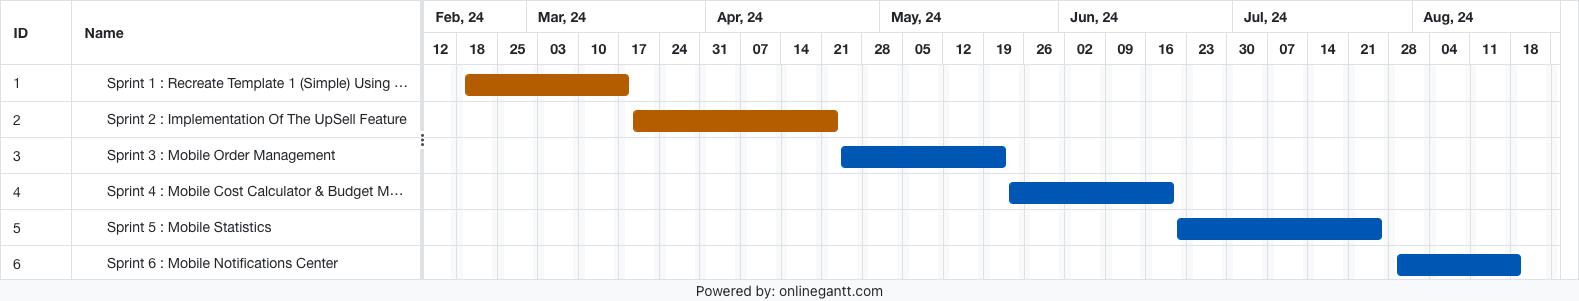
\includegraphics[width=1\textwidth]{Images/Online Gantt 20240715.png}
  \caption{Gantt Chart}
  \label{fig:Gantt Chart}
\end{figure}

\section{Conclusion}
In summary, this chapter outlined the scope of the project, detailing the host company, identified problems, and proposed solutions. The project aimed to optimize Converty's platform performance, add crucial features, and enhance the mobile app experience. The detailed management plan and timeline were presented to ensure effective project execution. By addressing the identified issues, the project aims to significantly improve Converty's functionality and user experience.
